\documentclass[a4paper]{article}
\usepackage[margin=1in]{geometry}

\usepackage[english]{babel}
\usepackage[utf8]{inputenc}
\usepackage{amsmath}
\usepackage{amsfonts}
\usepackage{natbib}
\usepackage{graphicx}
\usepackage[auth-sc,affil-sl]{authblk}
\usepackage[colorinlistoftodos]{todonotes}
\usepackage{hyperref}
\usepackage{enumitem}
\usepackage{pdfpages}
\usepackage{framed}

\addto{\captionsenglish}{\renewcommand{\abstractname}{Executive Summary}}

\title{Usability Test Report of CP's Website\\ (Proposal)}
\author[1]{Tested by: Luís  Cruz}
\affil[1]{MAP-i\\ Joint Doctoral Programme in Computer Science}
\date{Tested: January 20, 2014}



\begin{document}
\maketitle

Common Industry Format for Usability Test Report v1.1

Date prepared: January 27, 2014

Prepared by: Luís Cruz (luiscruz@fe.up.pt)

\begin{abstract}
vthe identity and a description of the product

va summary of the method(s) of the test including the number of and type of participants and their tasks.

vresults expressed as mean scores or other suitable measure of central tendency

w the reason for and nature of the test

w tabular summary of performance results.
\end{abstract}

\section{Introduction}
\subsection{Product Description}

CP.pt is the official website of emph{CP - Comboios de Portugal, E.P.E}, the public portuguese company responsible for rendering national and international passenger rail services.

CP customers vary according to the service provided. Many college students, workers and pensioners use the regional and urban services for small and medium distances. Long distance services are more used by college students that are away from home, tourists, and executive workers. Unfortunately, no official document stating the segmentation of the CP.pt website's users was found.

It is noticeable that CP services have a lot more passengers during school time, which means that students are an important segment of CP's customers. Besides, most of the students have good experience with the WEB, so the CP.pt website is expected to be a great tool to them. Therefore, this usability evaluation will focus in the segment of college students, which might be portuguese citizens as well as foreigners that study or want to study in Portugal and are able to speak English.

Many scenarios can apply for the use of the website by students. Some times they leave the classes earlier and need a way of quickly check if there are other alternative trains that can take them home earlier. Also sometimes there is no direct train to their destination, so they have to catch another in the the middle of the travelling. Another scenario is when the weekend is over and the student has to buy his/her ticket from home to his/her university city. Buying it from the website is more convenient since the student can avoid wasting time in the ticket lines and can grant a seat for his/her trip.

From the features implemented in the website, the following were tested:
\begin{itemize}
  \item Choose between Portuguese or English versions
  \item Check timetables for a trip.
  \item Buy fast train tickets, being the features that were tested.
\end{itemize}


\subsection{Test Objectives}

The aim of the test was to validate the usability of the main features of the CP.pt --- finding the most suitable train and buying tickets. It is important that these tasks are easy to learn.

Representative users were asked to complete some tasks, measures were taken of effectiveness, efficiency and satisfaction, and some notes about the users' opinion were taken in order to have ideas for some improvements that can be made.

\section{Method}

\subsection{Participants}

This test had 2 participants. Both were college students with ages between 21 and 26 years old. They are intermediate level users, that frequently use WEB applications. They already have experience in other transportation company's websites.

Students are used to get things fast and with an attractive design. Usually they have a laptop with a 13 or 15 inches screen, and use the 
Eduroam network when studying in the university.

\subsection{Context of Product Use in The Test}
\subsubsection{Tasks}
\label{sec:tasks}
The tasks that the participant has to accomplish are the following:

\begin{enumerate}
  \item Select the English Version of the application.
  \item Find the schedule for a trip from Braga to Aveiro.
  \item Find a cheap trip from Braga to Aveiro.
  \item Buy a ticket from Braga to Porto.
\end{enumerate}

These tasks are described in more detail in the \emph{Usability Test Plan}, available in the appendix~\ref{sec:usabilityTestPlan}. For each task, all the steps were defined in order to desscribe how the task can be efficiently accomplished.

These tasks were selected for being the features that are expected to be of the most important use. Every transportation website has these features and add great value to the customers, so it is important that they meet the users needs.

All the completion and performance criterias are also described in the Usability Test Plan (see appendix~\ref{sec:usabilityTestPlan}).

\subsubsection{Test Facility}

The test was made in a study room at the faculty. The moderator is sitting next to the participant in order to make the observation and query and give assistance. The screen and audio were recorded using the tool QuickTime Player 10.3 which is invisible to the user and does not affect the user experience.

\subsubsection{Participant’s Computing Environment}

According to \citep{http://www.satya-weblog.com/2013/07/desktop-laptop-mobile-screen-resolution-most-common-worldwide.html}, the most common resolution used in WEB is $1366\times 768$. In this experiment a 13 inches RGB screen with approximately the same resolution was used: $1440\times 990$. For interaction with the application the participant used an Apple laptop keyboard, and an Apple Magic mouse. Some other devices were available if the user didn't feel comfortable with these devices, however, they were not used.

The browser Safari 7.0.1 with default settings was used with an internet connection which had an average download and upload speeds of $4 Mbit/s$ and $1Mbit/s$, respectively.


\subsubsection{Test Administrator Tools}

A \emph{Data Logging Form} (see ~\ref{sec:dataLoggingForm}) was designed providing the moderator with a tool to record some notes about each task of each participant. The form has some variables \todo{define variables}, and a generic questionnaire to be asked to the user. It also provides a space to take some notes while the moderator conducts a small post-task interview.

All the task information is provided in the \emph{Usability Test Plan}, available in the appendix~\ref{sec:usabilityTestPlan}, defining a script about how the moderator should conduct the experiment is provided. All the steps that are necessary to finish a task are clearly described as well as some guidelines with the important questions for the post-task interview.

After the test, the participants were asked to answer a post-test questionnaire based on~\citep{} provided in appendix~\ref{sec:postTestQuestionnaire}.

As it was already mentioned, during the experiments, the screen and voice were recorded using the tool QuickTime Player 10.3.

\subsection{Experimental Design}
vDescribe the logical design of the test. Define independent variables and control variables. Briefly describe the measures for which data were recorded for each set of conditions. \todo{vriables}

\subsubsection{Procedure}

The participants were informed that the usability of CP's website was being tested, to find out whether it met the needs of users such as themselves. They were told that it was not a test of their abilities. They were asked to sign a consent form.

Participants were given introductory instructions. The evaluator reset the state of the computer before each task, and provided instructions for the next task. 

The participant could ask for assistance and make questions whenever they find necessary, in order clarify any part of the task. All assistances were logged by the moderator. Also there was no time limit for the task completions, but if the moderator feels that the participant is stuck in some part, he was allowed to give some hints if properly logged.

After each task the moderator conducted a small interview trying to answer some crucial questions provided in the Usability Test Plan (see appendix~\ref{sec:usabilityTestPlan}).

The participants were non remunerated voluntaries and during each test session only the moderator and a participant were present.

\subsubsection{Participant General Instructions}

The instructions were given personally by the moderator to each participant. The test session proceeds by having only one user in the room with a moderator. Whenever the user needed help he/she could simply ask for help.
 The participant was asked to use the \textit{think-aloud} technique, describing every step he/she makes during the tasks. The moderator will be directly observing the participant and taking some notes using the Data Logging Form, provided in appendix~

\subsubsection{Participant Task Instructions}
Before starting each task the moderator explained what it was expected to accomplish in the following task. The task instructions are very simple, being described in a short sentence, as stated in section~\ref{sec:tasks}.

\subsection{Usability Metrics}
vExplain what measures have been used for each category of usability metrics: effectiveness, efficiency and satisfaction. Conceptual descriptions and examples of the metrics are given below.

\subsubsection{Effectiveness}
For measuring effectiveness the following measures were considered:
  \begin{description}
    

    \item[Completion Rate] the percentage of participants that correctly finished each task.
 \item[Unassisted Completion Rate] the percentage of participants that correctly finished each task without assistance.
 \item[Number of Assistances] The average of assurances given in each task.
 \item[Back Button hits] The average of times the user hit the Back Button in the browser.
 \item[Errors] The number of times a user had to repeat parts of the task.
  \end{description} 
 
 \subsubsection{Efficiency}
 Efficiency was accessed by measuring the following parameters:
\begin{description}  

  \item[Task time] The average time the users took to correctly complete each task.
 \item[Completion rate efficiency] mean completion rate/mean task time.
\end{description} 
 
 \subsubsection{Satisfaction}
 Satisfaction is a subjective measure that correlates with the user's motivation to use a product. The standardized instrument \textit{System Usability Scale} (SUS) provides a 10 item questionnaire with five-scale responses that can be converted into a score.\todo{reference SUS} After the test the users answered this questionnaire. 
 
 Also a post-test questionnaire based on \todo{http://www.w3.org/WAI/redesign/ut\_report/appendices.html} was given to the participants (available in appendix~\ref{sec:post_questionnaire}). This questionnaire intended to provide some insights about the way the design should be changed to make it more suitable to the user.
 
 
 \section{Results}
 \subsection{Data Analysis}
 \subsubsection{Data Scoring}
 The method by which the data collected were scored should be described in sufficient detail to allow replication of the data scoring methods by another organization if the test is repeated. Particular items that should be addressed include the exclusion of outliers, categorization of error data, and criteria for scoring assisted or unassisted completion.
  \subsubsection{Data Reduction}
  The method by which the data were reduced should be described in sufficient detail to allow replication of the data reduction methods by another organization if the test is repeated. Particular items that should be addressed include how data were collapsed across tasks or task categories.
   \subsubsection{Statistical Analysis}
   
   \subsection{Presentation of the Results}
   Effectiveness, Efficiency and Satisfaction results must always be reported

\subsubsection{Performance Results}
TABLE

\appendix

\section{Consent and Recording Release Form}
\todo{reference}
\begin{oframed}
  \begin{center}
    \large \textsc{Consent and Recording Release Form}}
  \end{center} 
I agree to participate in the study conducted and recorded by the MAP-i student Luís Cruz. 

I understand and consent to the use and release of the recording by Luís Cruz. I understand that the information and recording is for research purposes only and that my name and image will not be used for any other purpose. I relinquish any rights to the recording and understand the recording may be copied and used by Luís Cruz without further permission. 

I understand that participation in this usability study is voluntary and I agree to immediately raise any concerns or areas of discomfort during the session with the study administrator.

Please sign below to indicate that you have read and you understand the information on this form and that any questions you might have about the session have been answered. 

~

Date: \rule{2cm}{0.4pt} 

Please print your name: \hrulefill

Please sign your name: \hrulefill



Thank you!

Your participation is kindly appreciated.
\end{oframed}

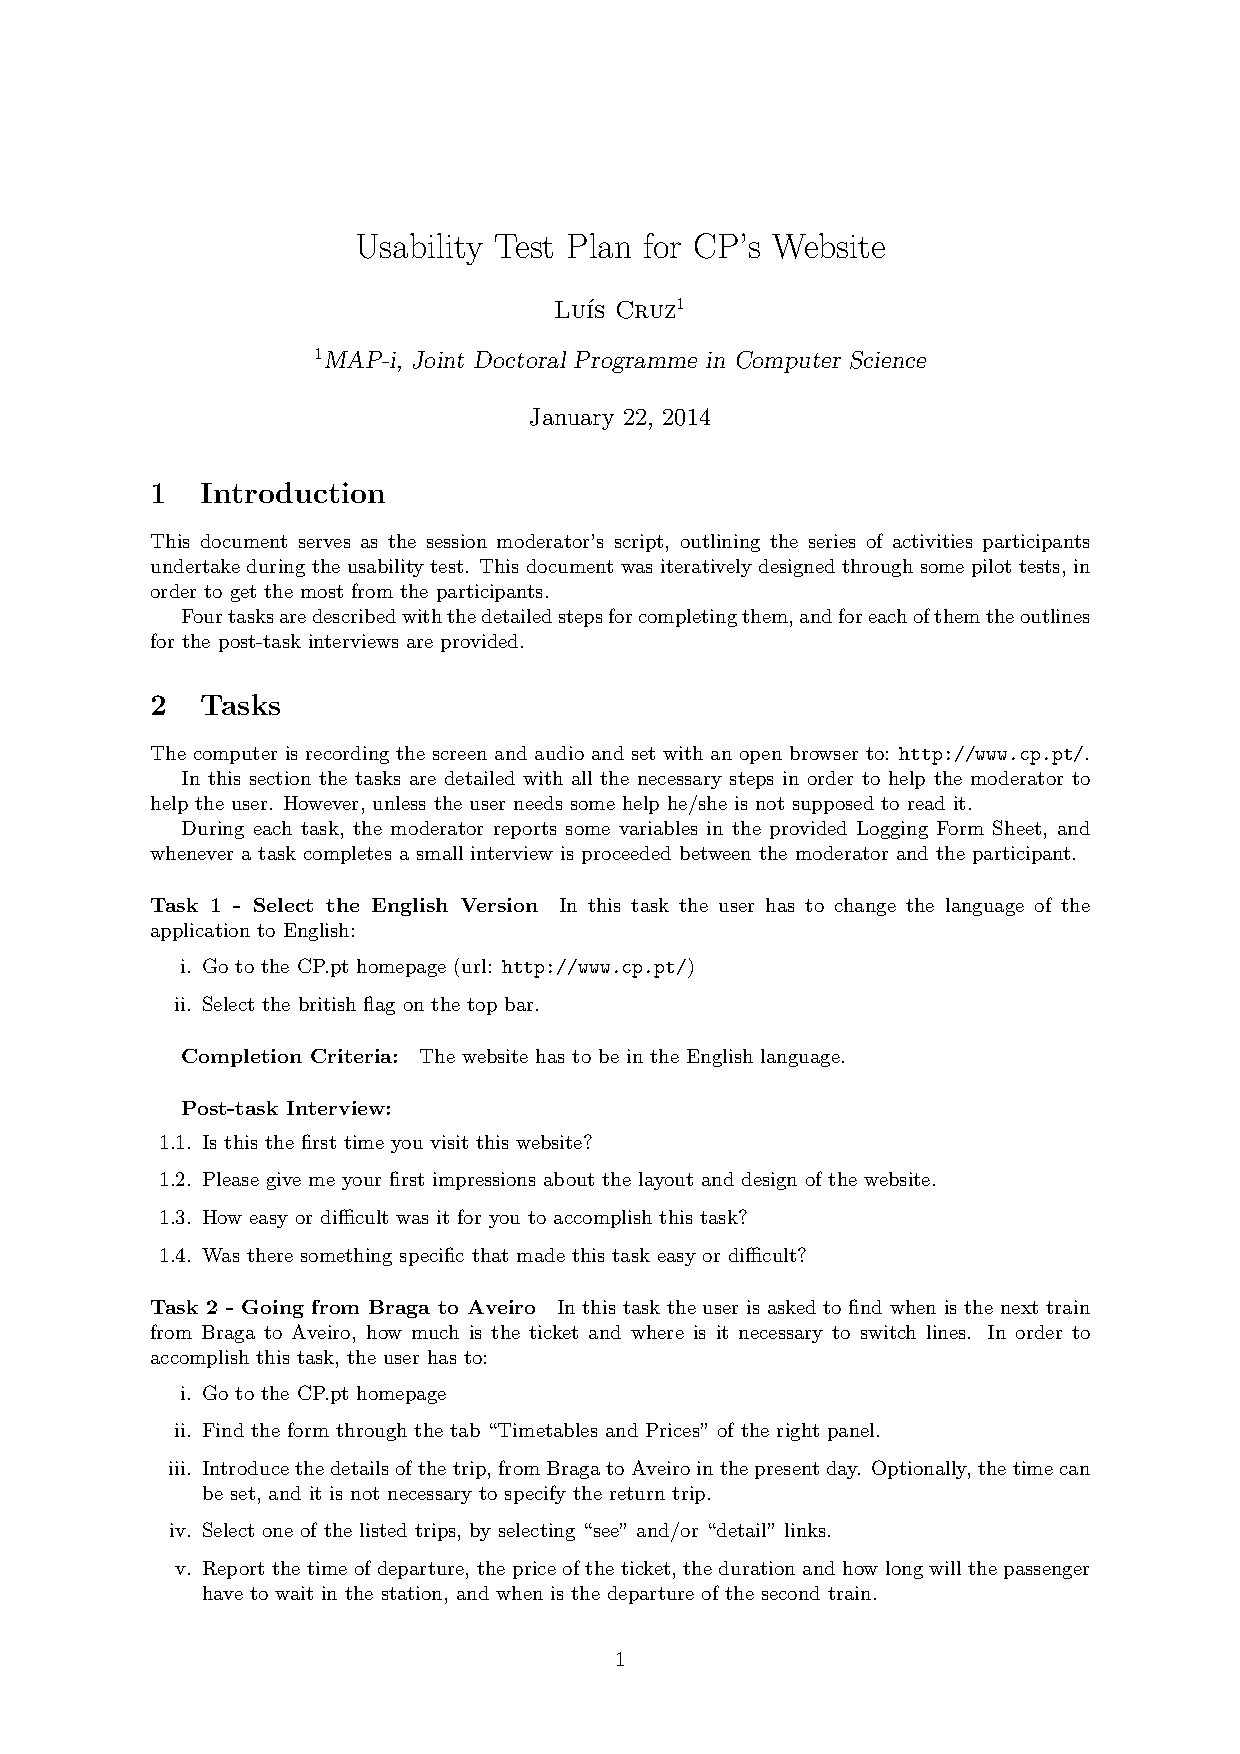
\includepdf[pagecommand=\section{Usability Test Plan}\label{sec:usabilityTestPlan}\thispagestyle{plain}{The plain original document can be accessed at \url{http://paginas.fe.up.pt/~luiscruz/cp_usability/}}, nup=2x2, pages=-, frame=true, scale=0.78, offset=0 -25]{../usabilityTestPlan/master.pdf}

% ------- DATA LOGGIN FORM -------- %

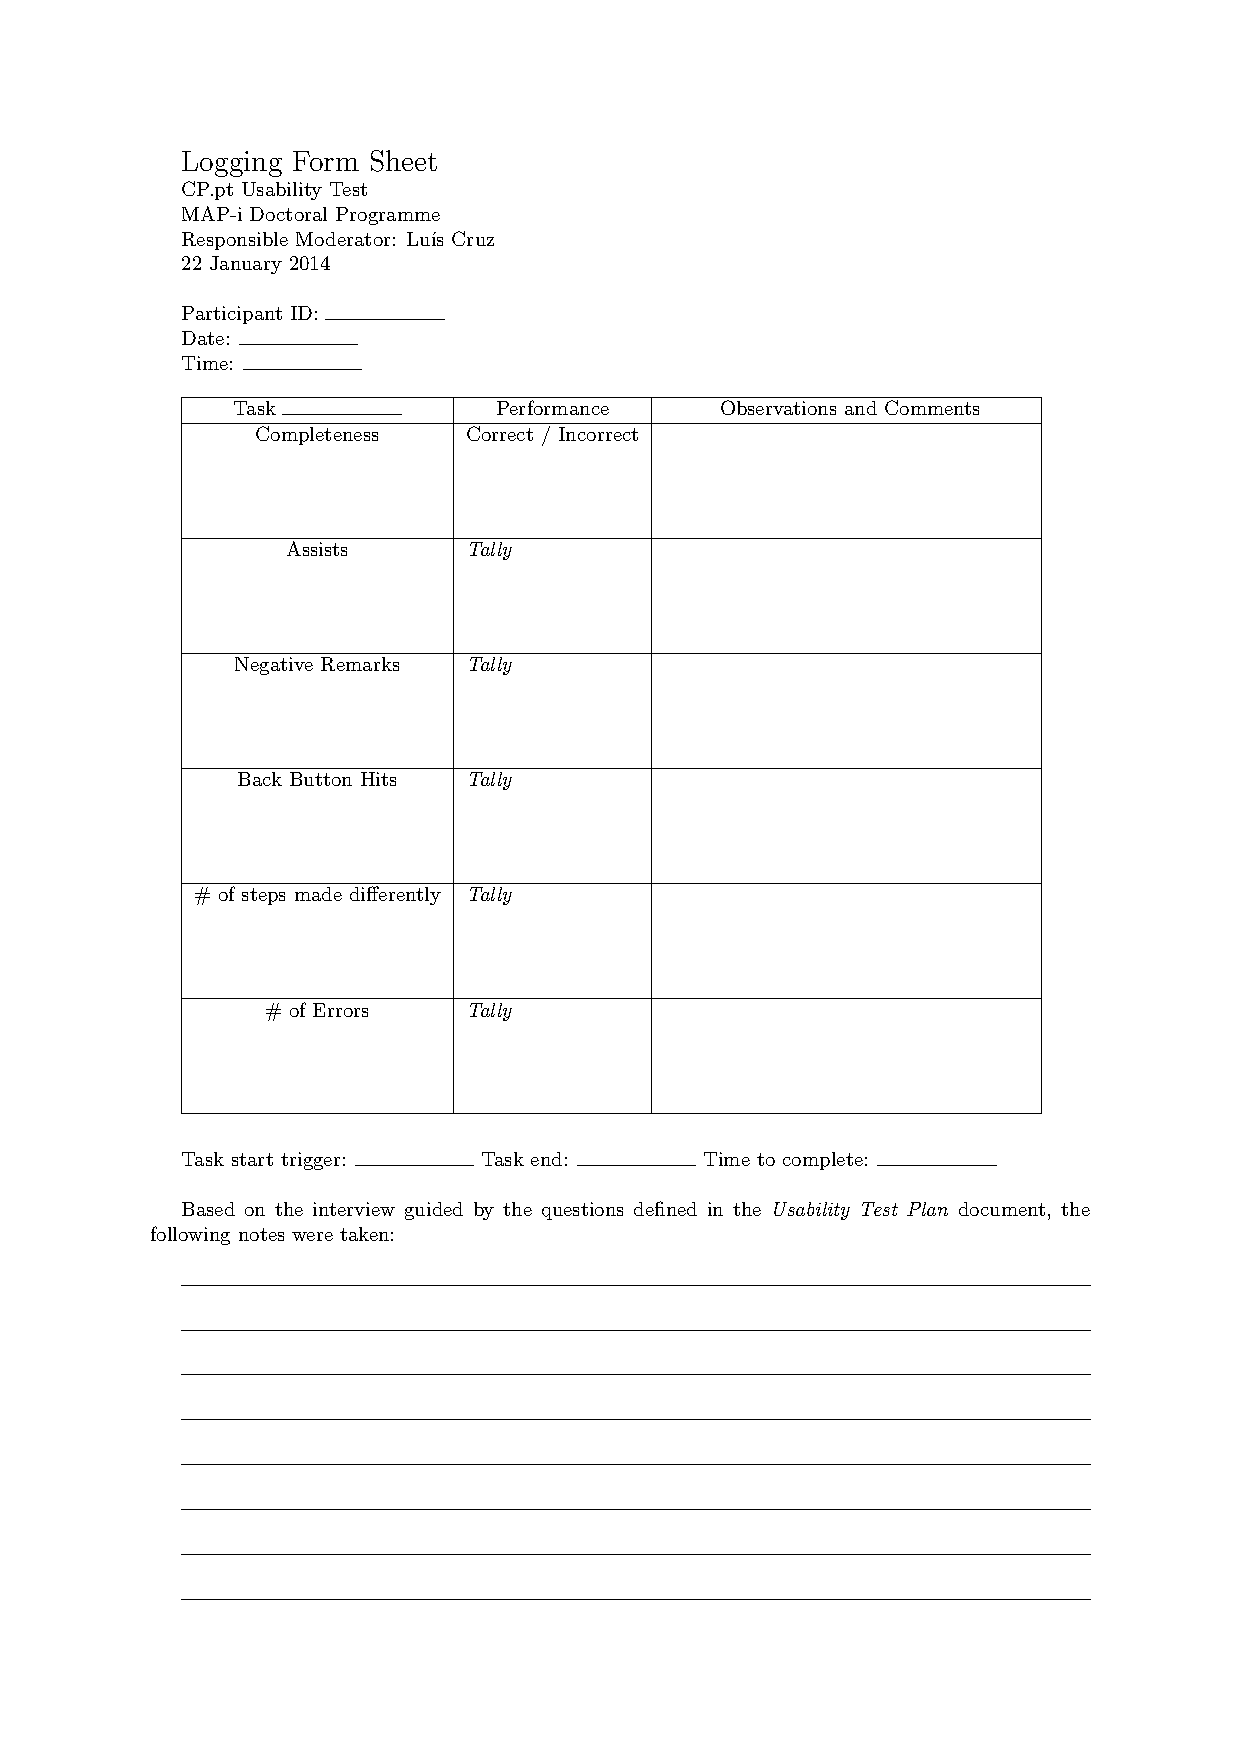
\includepdf[pagecommand=\section{Data Logging Form}\label{sec:dataLoggingForm}\thispagestyle{plain}{The moderator of the usability test observes the behavior of the participant while taking notes in the Data Logging Form. Each task needs one Data Logging Form.}, pages=-, frame=true, scale=0.75, offset=0 -25]{../dataLoggingForm/master.pdf}


% ---------------~o~--------------- %

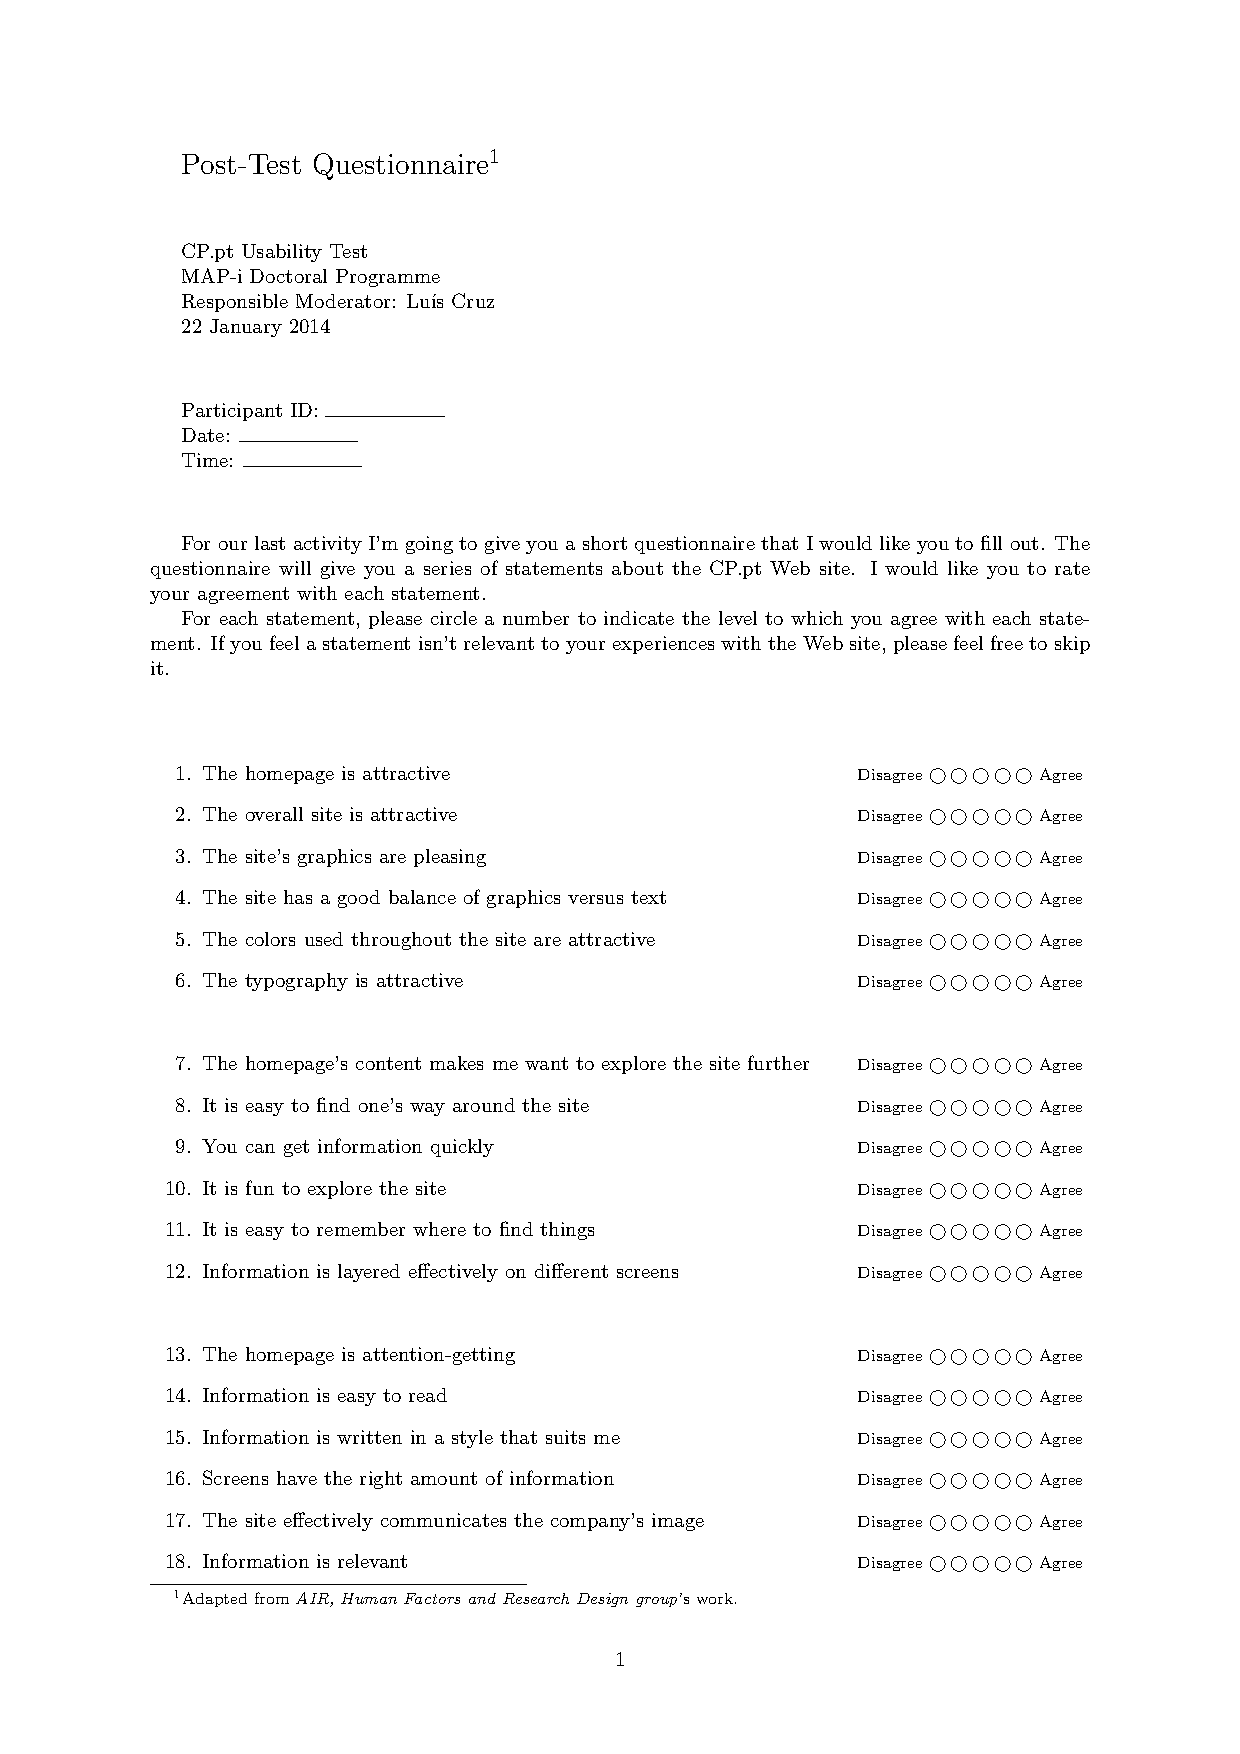
\includepdf[pagecommand=\section{Post-Test Questionnaire}\label{sec:postTestQuestionnaire}\thispagestyle{plain}{The moderator of the usability test observes the behavior of the participant while taking notes in the Data Logging Form. Each task needs one Data Logging Form.}, pages=1, frame=true, scale=0.75, offset=0 -25]{../postTestQuestionnaire/master.pdf}
\includepdf[pagecommand=\thispagestyle{plain}, pages=2-, frame=true, scale=0.75, offset=0 0]{../postTestQuestionnaire/master.pdf}
%----------------------------------------------------------------------------------------
%	BIBLIOGRAPHY
%----------------------------------------------------------------------------------------

\bibliographystyle{apalike}
\bibliography{../bibliography}

%----------------------------------------------------------------------------------------

\end{document}